\documentclass{article}
\usepackage{fontspec}
\usepackage{graphicx}
\usepackage{amssymb}
\usepackage{wasysym}
\usepackage{enumitem}
\usepackage{fontawesome5}

\usepackage[margin=1.5cm]{geometry}

\setmainfont{Arial}
\parindent0mm
\linespread{1.2}

\begin{document}
\pagenumbering{gobble}

\vspace*{\fill}

\begin{figure}[tph!]
\centering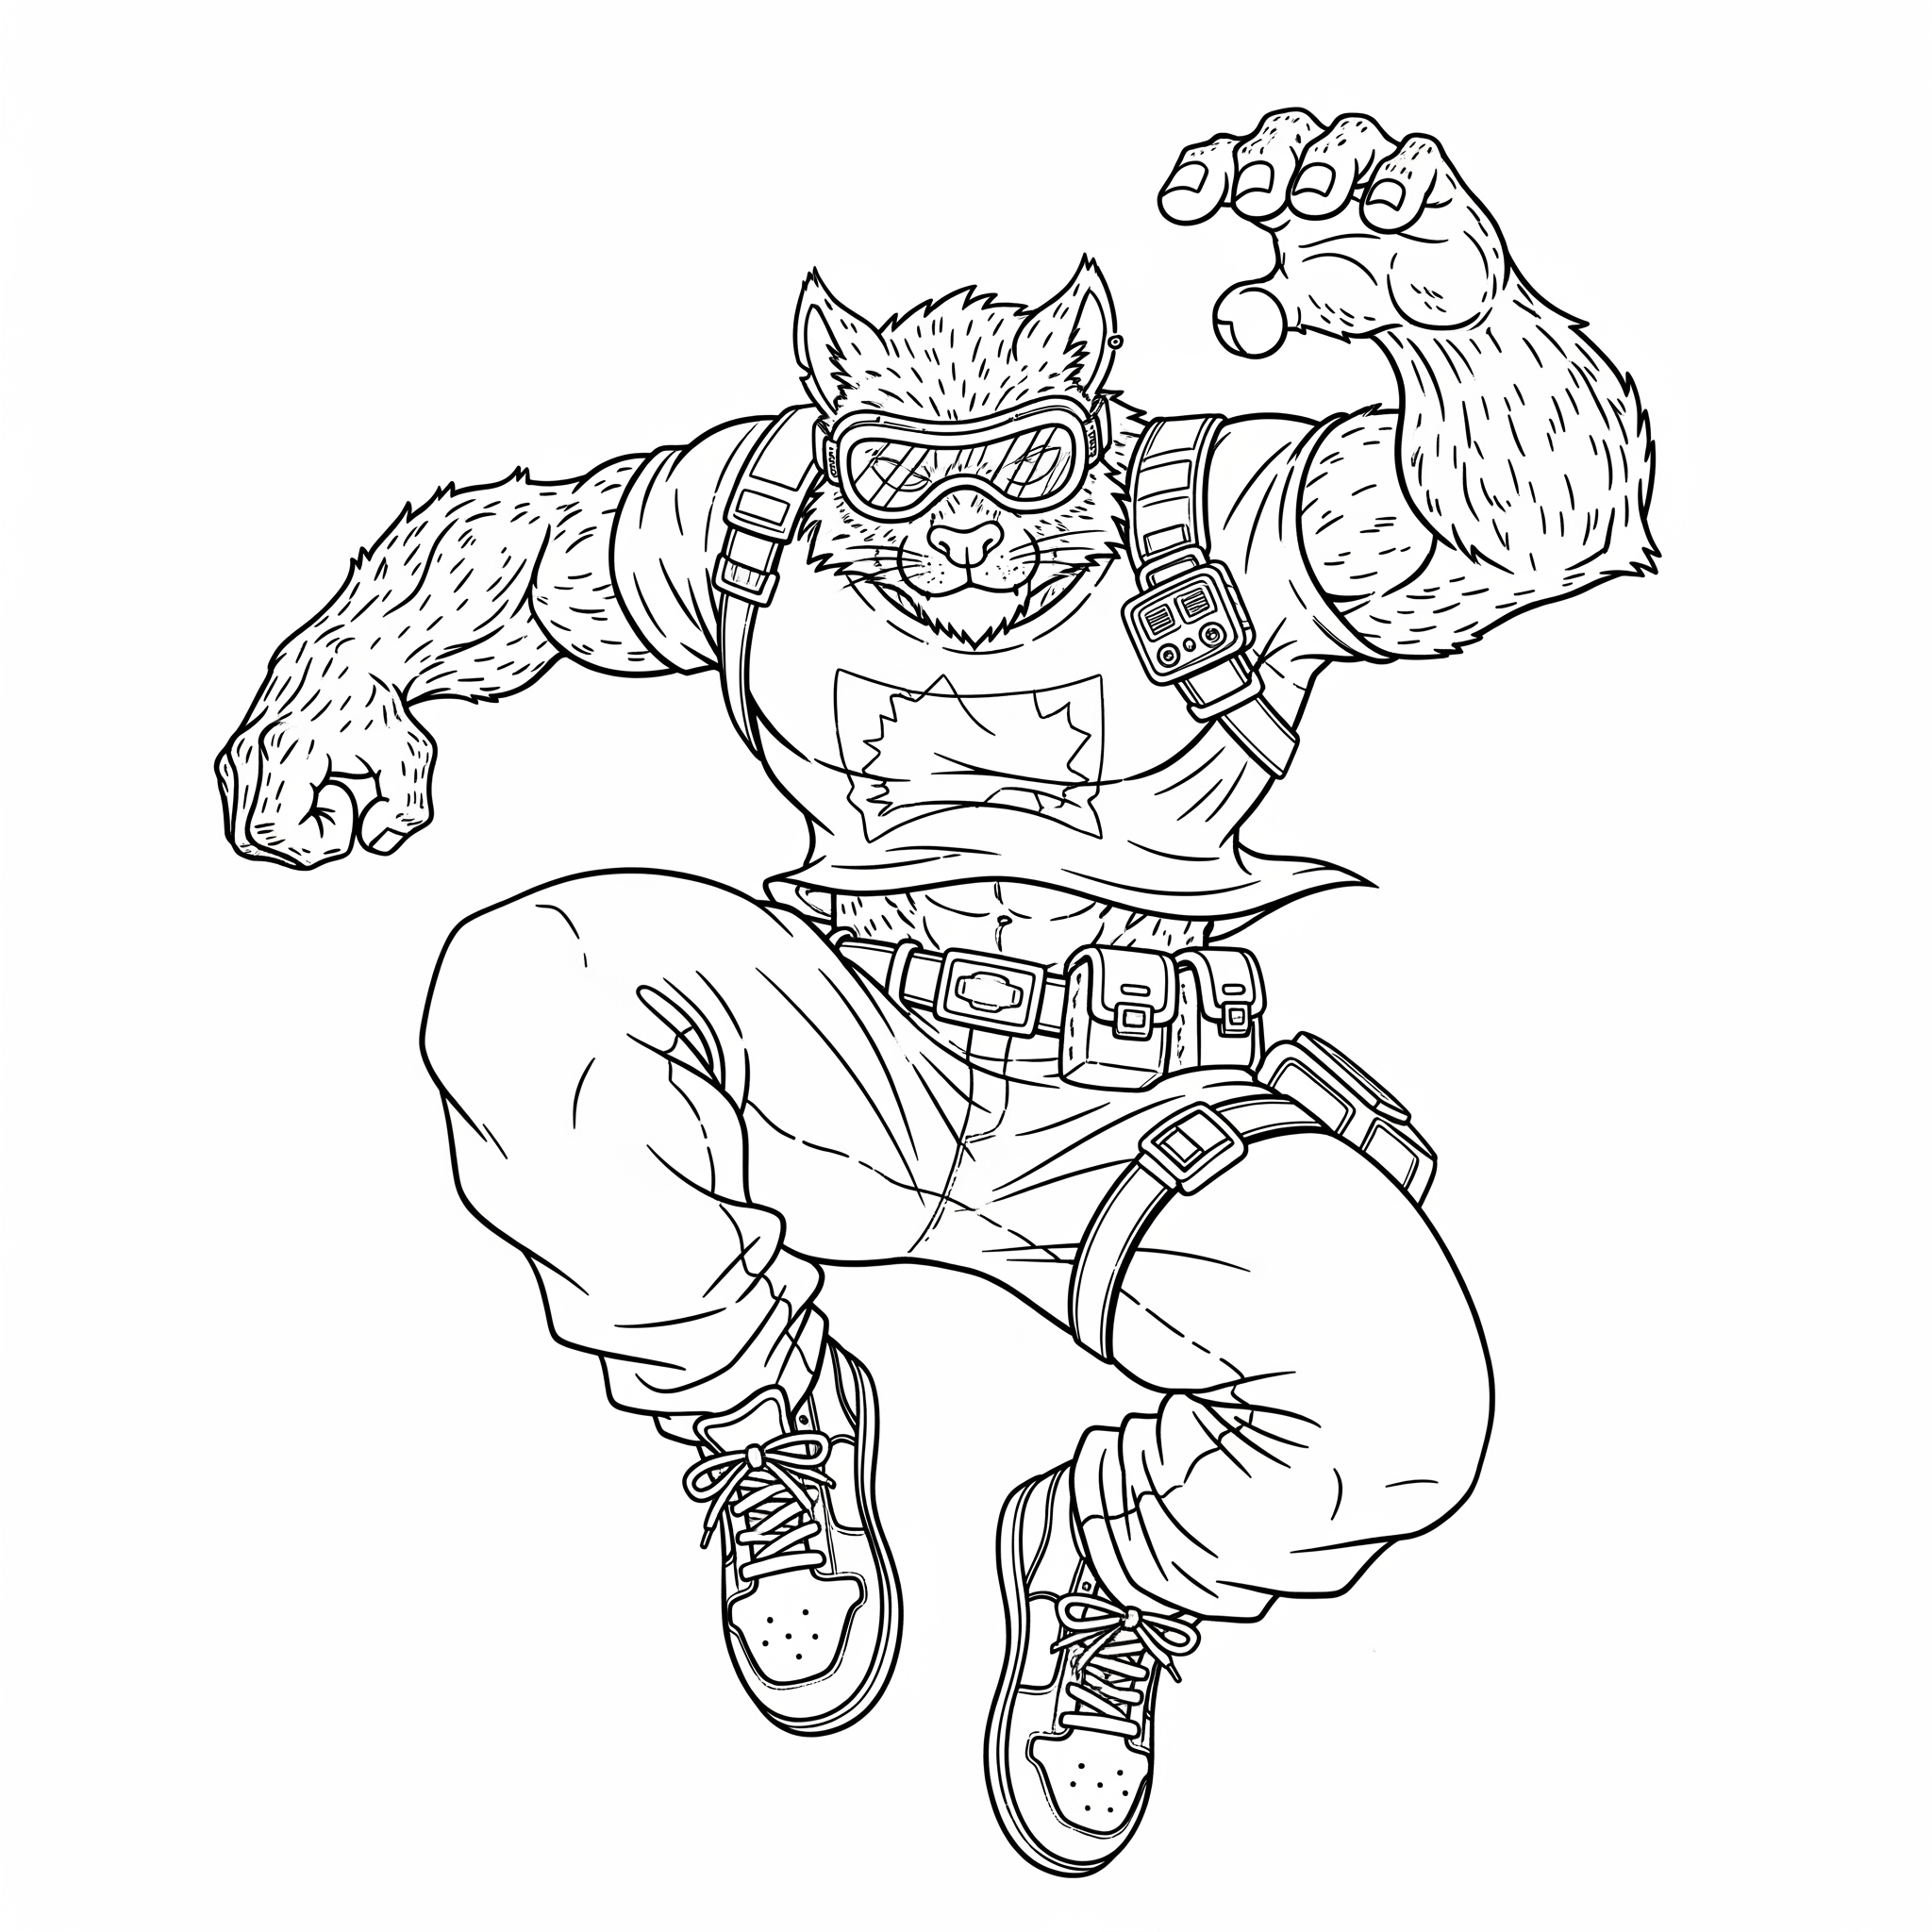
\includegraphics[width=12cm]{images/frontCover.png}
\end{figure}
\centering\Huge\fontspec{TradeWinds-Regular.ttf}Martial Mutant Misfitz!

\newpage
\pagenumbering{arabic}

\section*{\fontspec{TradeWinds-Regular.ttf}What is Martial Mutant Misfitz?}
\raggedright\normalfont\large You are humanoid animal mutants. Human society rejects you. Your appearance is alien and off-putting to most humans. Fortunately, a mentor came into your life. Taking care of you when you needed it the most. Training you in martial prowess, and teaching you how to leverage your new abilities. A mentor hiding your from society and shielding you from harm. But this could soon end, as a new evil rises, that threatens the city. Who is gonna stop it? Who if not you?!

Martial Mutant Misfitz is a game about whacky teenagers mutated into animals. It's a game about stylish fighting and kung fu. It also is a game about being an outsider --- he feeling of not fitting into society. And lastly, it's a game about family.
\newpage
\pagenumbering{gobble}

\vspace*{\fill}

\begin{figure}[h!]
\centering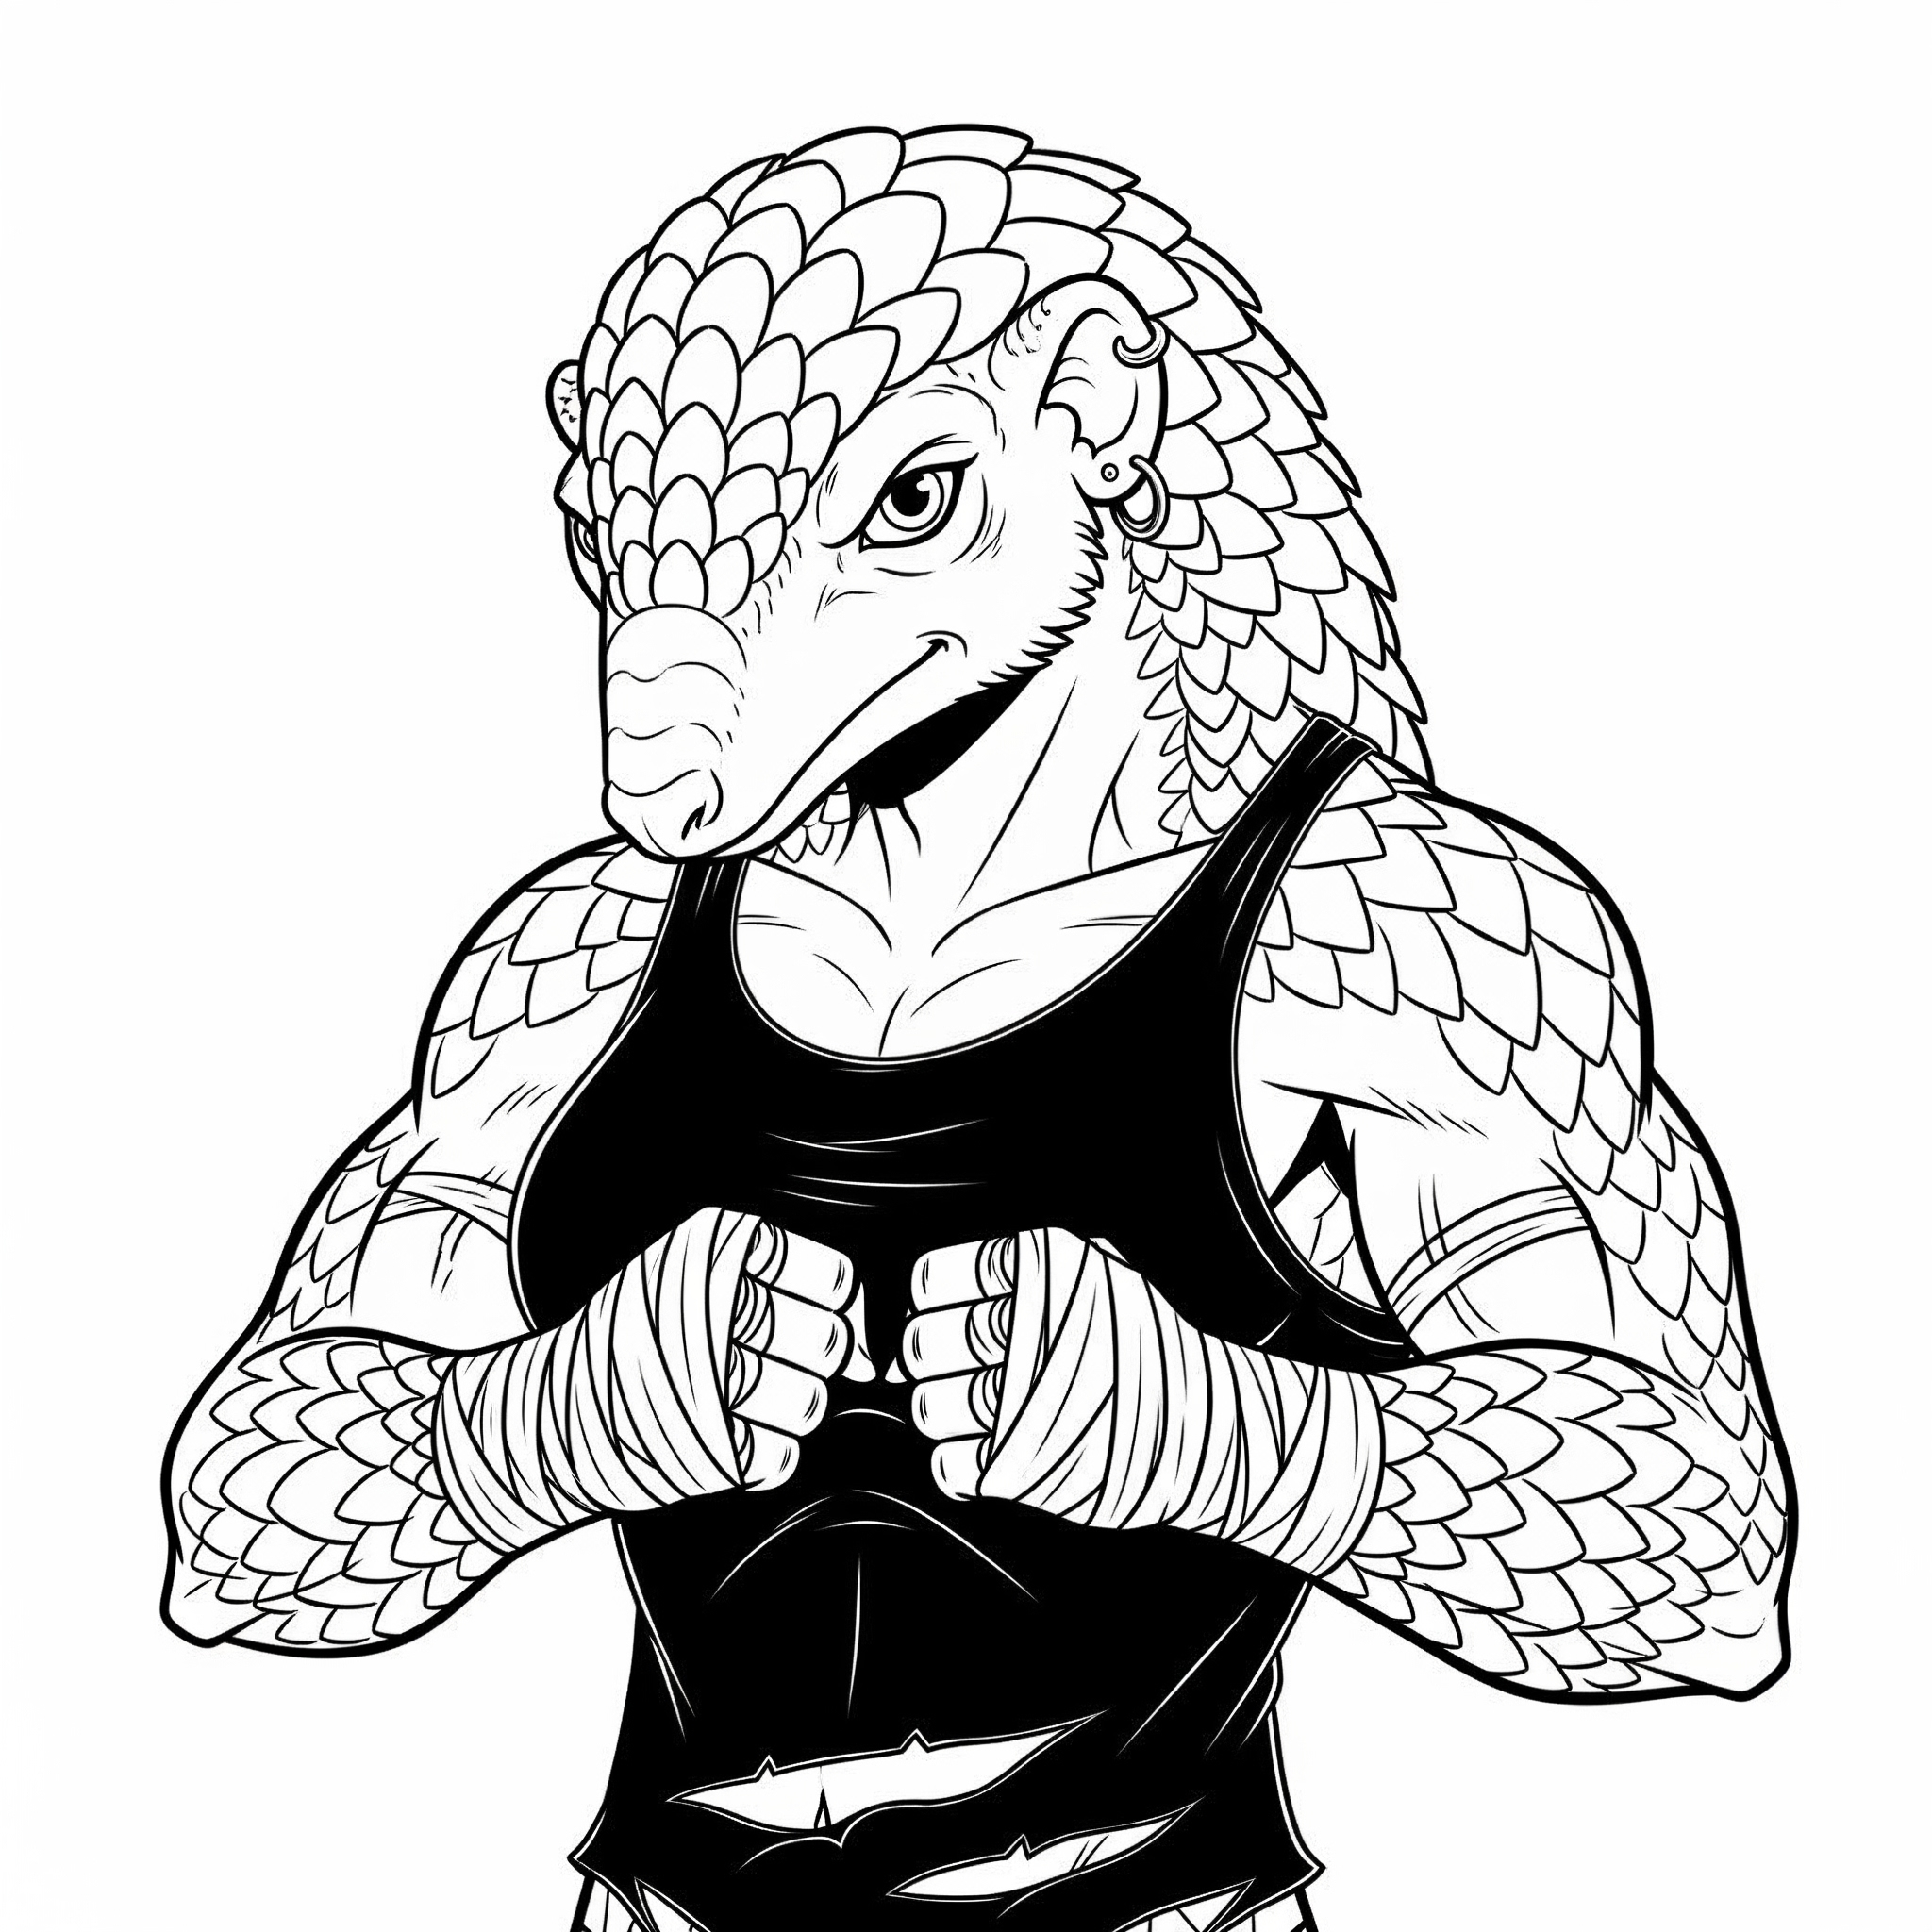
\includegraphics[width=12cm]{images/brawler.png}
\vspace{-\baselineskip}\vspace{+0.1pt}
\rule{\linewidth}{2pt}
\end{figure}
\Huge\fontspec{TradeWinds-Regular.ttf}The Brawler

\normalfont\large
\medskip

Big muscles, bigger attitude. Always ready to rumble.

\medskip

You love fighting and your mutations gave you the tools to really excel at it. This gives you the power to protect others. However, your hot headedness brings you a lot of trouble.

\newpage

\Large\fontspec{TradeWinds-Regular.ttf}Animal

\medskip

\normalfont\large 1.Bear, 2.Rhino, 3.Buffalo, 4.Crocodile, 5.Kangaroo, 6.Pangolin, \rule{2cm}{1pt}

\medskip

\Large\fontspec{TradeWinds-Regular.ttf}Names

\medskip

\normalfont\large 1.Knuckles, 2.Jax, 3.Brock, 4.Roxy, 5.Bruiza, 6.Wrecka, \rule{2cm}{1pt}

\medskip

\Large\fontspec{TradeWinds-Regular.ttf}Enhancements

\medskip

\normalfont\large Pick or roll two:

\(\square\) \textbf{Electrified Brass Knuckles} (2 harm, 1 harm ignores armor, hand)

\(\square\) \textbf{Spiked Wrist Wraps} (1 harm, quick, hand)

\(\square\) \textbf{Tech-Spine} (makes all weapons quick)

\(\square\) \textbf{Hardened Skin} (2 armor vs. piercing)

\(\square\) \textbf{Razor Claws} (2 harm, messy, hand)

\(\square\) \textbf{Steel Bones}  (2 armor vs. blunt)

\medskip

\Large\fontspec{TradeWinds-Regular.ttf}Advancements \(\LARGE \Circle \Circle \Circle \Circle \Circle \)

\medskip

\normalfont\large

\begin{tabular}{l @{\hspace{2cm}} l}
\(\square\) Get +1 Power, max +3 & \(\square\) Take another Brawler move \\
\(\square\) Get +1 Cool, max +3 & \(\square\) Take another Brawler enhancement \\
\(\square\) Get +1 Wits, max +3 & \(\square\) Take a move from another playbook \\
\(\square\) Get +1 Heart, max +3 & \(\square\)  Take a move from another playbook \\
\(\square\) Get +1 Weird, max +3 & \\
\end{tabular}

\medskip

\Large\fontspec{TradeWinds-Regular.ttf}Conditions

\medskip

\normalfont\large

\(\square\) \textbf{Exposed} (-2 to Power until you eliminate or evade the skeptical)\\
\(\square\) \textbf{Angry} (-2 to Cool until you hurt someone or break something)\\
\(\square\) \textbf{Stressed} (-2 to Weird until you say sth hurtful to someone)\\
\(\square\) \textbf{Jealous} (-2 to Heart until you go on an ego trip)\\
\(\square\) \textbf{Insecure} (-2 to Charm until you take a comment to wrong way)\\
\(\square\) \textbf{Poisoned}  (-1 to all stats until healed)

\medskip

\Large\fontspec{TradeWinds-Regular.ttf}Harm \(\bigtriangledown \bigtriangledown \bigtriangledown \bigtriangledown | \bigtriangledown \bigtriangledown\)

\medskip

\Large\fontspec{TradeWinds-Regular.ttf}Stats

\normalfont\Huge

\faBomb \faStar \faHeart \faBrain \faPizzaSlice \faCircle[regular]

\medskip

\Large\fontspec{TradeWinds-Regular.ttf}Notes

\newpage

\Large\fontspec{TradeWinds-Regular.ttf}Brawler Moves

\medskip

\normalfont\large

\begin{itemize}[label=$\square$]

\item \textbf{One more word and I break your nose} If you try to provoke or intimidate someone you can roll + Power on Talk the Talk

\item \textbf{Nothin’ But a Scratch} Once per session you can roll + Cool. On a 10+ heal 2 harm and stabilize your wounds. On a 7-9 you may stabilize or heal 1 harm. On a miss, it was worse than it looked

\item \textbf{Walls are optional} Break through walls, destroy or throw obstacles. On a hit, choose one of the following:
\vspace{-6pt}
\begin{itemize}
    \setlength\itemsep{-0.5em}
\item Deal 2 harm
\item Get or give +1 forward
\item You draw attention - enemies focus on you.
\item You create a advantageous position for your team.
\end{itemize}
\vspace{-6pt}
On a 7-9 additionally choose one of the following:
\vspace{-6pt}
\begin{itemize}
    \setlength\itemsep{-0.5em}
\item  Take 1 harm
\item  Take 1 condition
\end{itemize}

\item \textbf{Coming through!} When you charge at the enemy, you shrug off harm until your momentum stops.

\item \textbf{You brought a gang? Cute.} Once per session, you can add area to any attack.

\end{itemize}


\Large\fontspec{TradeWinds-Regular.ttf}Relations

\medskip

\normalfont\large

\begin{itemize}[label=$\square$]
    \item \rule{2cm}{1pt}’s and my fighting style derived from the same base style. How is it called? What does it look like? What is it about?
    \item I often get into trouble with \rule{2cm}{1pt}. Doing what?
    \item When we were younger, \rule{2cm}{1pt} and I wrestled all the time. What famous wrestler did you play?
\end{itemize}

\begin{tabular}{l @{\hspace{2cm}} l}

\Large\fontspec{TradeWinds-Regular.ttf}Leading Principles & \Large\fontspec{TradeWinds-Regular.ttf}Flipside \\

\normalfont\large

$\bullet$ Protect others & $\bullet$ Risk too much \\
$\bullet$ Take Action &  $\bullet$ Be impatient \\
$\bullet$ Go solo &  $\bullet$ Freak out way too soon \\
$\bullet$ Take an ego trip &  $\bullet$ Think too little about a plan or problem \\

\end{tabular}


\end{document}